\scanpage{136}
that $G\mathrm{x}V\handwritten{\longrightarrow}V\mathrm{x}V$ is a monomorphism (this is Nakayama's lemma), and it is then well known (SGA 3 $\mathrm{VII}_{\mathrm{B}}$ ...) that \deleted{$V$ is a} one has a nice quotient $W=V/G$, with $\deleted{W\quad V}$ $V\handwritten{\longrightarrow}W$ flat and in fact the structure projection of a $G_{W}$-torsor. Of course the coalgebra $\overset{\handwritten{-}}{M}$ is none other than the one defining the preceding quotient $W$. In general, there is no question of proving that $V\handwritten{\simeq}W\mathrm{x}G$ as a formal variety with operators (i.e. that the preceding torsor is trivial), i.e. of finding a\deleted{isomorphism} section of $V$ over $W$, i.e. a comodule lifting $\overset{\handwritten{-}}{M}\handwritten{\longrightarrow}M$; one can only say that any lifting as $k$-vector spaces will define an isomorphism $A\otimes_{k}\overset{\handwritten{-}}{M}\handwritten{\simeq}M$ of $A$-modules. However, if $G$ is formally smooth i.e. the dual of $A$ an algebra of formal power \rlap{p}series (possibly with an infinite number of generators) then one will have perfect splitting; this will be the case in particular in characteristic zero.

\uline{Example} 2. Suppose $A$ commutative with respect to its algebra law. Thus $A$ is the affine algebra of an 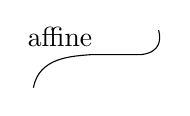
\begin{tikzpicture}[baseline=-.6ex,x=1cm,y=1cm]
\node[anchor=west,inner sep=0] at (0,.42) {\inserted{affine}};
\draw (.08,-.22) .. controls (.15,.16) and (.55,.18) .. (.82,.2) -- (1.45,.2) .. controls (1.7,.23) and (1.7,.4) .. (1.67,.51);
\end{tikzpicture} monoid scheme $G$. The hypothesis on the coc\deleted{c}omplete filtration is rather strange here, it is stated by saying that for every $f\handwritten{\in}A$ (function on $G$) \deleted{vanishing at $e$}, there exists an integer $n$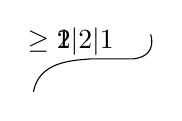
\begin{tikzpicture}[baseline=-.6ex,x=1cm,y=1cm]
\node[anchor=west,inner sep=0] at (0,.42) {\inserted{$\handwritten{\geq\unsure{\rlap{\(1\)}2|2|1}}$}};
\draw (.08,-.22) .. controls (.15,.16) and (.55,.18) .. (.82,.2) -- (1.35,.2) .. controls (1.6,.23) and (1.6,.4) .. (1.57,.51);
\end{tikzpicture} such that the function in $n$\deleted{\unsure{s|x}} variables $f(g_{1}g_{2}\cdots g_{n})$ is \deleted{identically zero}\inserted{a sum of functions} in $n-1$ of the var\rlap{a}i\rlap{a}ibles.\margin{\figure{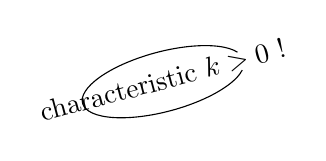
\begin{tikzpicture}[rotate=15,transform shape]
\node[inner sep=3pt] (n) {\handwritten{characteristic $k>0$ !}};
\draw (1.01,.10) arc[start angle=18,end angle=342,x radius=1.06cm,y radius=.38cm];
\end{tikzpicture}}} If $G$ is of finite type over $k$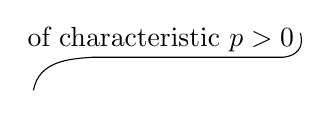
\begin{tikzpicture}[baseline=-.6ex,x=1cm,y=1cm]
\node[anchor=west,inner sep=0] at (0,.42) {\inserted{\handwritten{of characteristic $p>0$}}};
\draw (.08,-.22) .. controls (.15,.16) and (.55,.18) .. (.82,.2) -- (3.25,.2) .. controls (3.5,.23) and (3.5,.4) .. (3.47,.51);
\end{tikzpicture}, I think that \deleted{as soon as one replaces one of the variables in it by $1$, but then, making all} this must entai\rlap{t}l that \deleted{the identity of} $G$ is \figure{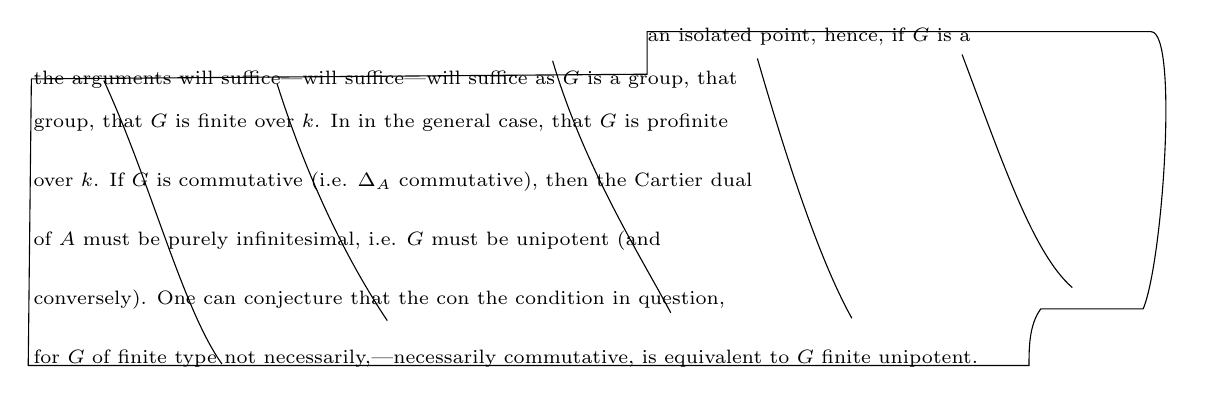
\begin{tikzpicture}[x=1cm,y=1cm,every node/.style={anchor=base west,inner sep=0,font=\scriptsize}]
\node at (7.8,0) {\deleted{an isolated point, hence, \deleted{if $G$ is a}}};
\node at (0,-0.55) {\deleted{\deleted{the arguments \unsure{will suffice|will suffice|will suffice}} as $G$ is a group, that}};
\node at (0,-1.1) {\deleted{\deleted{group, that} $G$ is finite over $k$. \deleted{In in the general case, that $G$ is profinite}}};
\node at (0,-1.85) {\deleted{\deleted{over $k$.} If $G$ is commutative (i.e. $\handwritten{\Delta}_{A}$ commutative), then the Cartier dual}};
\node at (0,-2.6) {\deleted{of $A$ must be purely infinitesimal, i.e. $G$ must be unipotent (and}};
\node at (0,-3.35) {\deleted{conversely). One can conjecture that \deleted{the con} the condition in question,}};
\node at (0,-4.1) {\deleted{for $G$ of finite type not \unsure{necessarily,|necessarily} commutative, is equivalent to $G$ finite unipotent.}};
\draw (7.8,.12) -- (14.2,.12) .. controls (14.55,.12) and (14.35,-2.8) .. (14.1,-3.4) -- (12.8,-3.4) .. controls (12.65,-3.6) and (12.65,-3.9) .. (12.65,-4.12) -- (-.06,-4.12) -- (-.02,-.48) -- (7.8,-.42) -- cycle;
\draw (.9,-.50) .. controls (1.5,-1.8) and (1.9,-3.4) .. (2.4,-4.10);
\draw (3.1,-.54) .. controls (3.5,-1.8) and (4.0,-2.8) .. (4.5,-3.55);
\draw (6.6,-.25) .. controls (7.0,-1.6) and (7.7,-2.7) .. (8.1,-3.45);
\draw (9.2,-.22) .. controls (9.6,-1.6) and (10.0,-2.8) .. (10.4,-3.52);
\draw (11.8,-.17) .. controls (12.3,-1.5) and (12.7,-2.7) .. (13.2,-3.13);
\end{tikzpicture}}\margin{\handwritten{?}}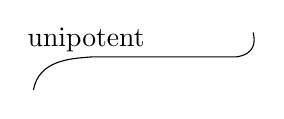
\begin{tikzpicture}[baseline=-.6ex,x=1cm,y=1cm]
\node[anchor=west,inner sep=0] at (0,.42) {\inserted{\handwritten{unipotent}}};
\draw (.08,-.22) .. controls (.15,.16) and (.55,.18) .. (.82,.2) -- (2.65,.2) .. controls (2.9,.23) and (2.9,.4) .. (2.87,.51);
\end{tikzpicture} so if one no longer assumes $G$ of finite type either, that $G$ is \deleted{profinite and} prounipotent.

% archive sheet number: 135
